\documentclass[12pt,a4paper]{article}

% ── Packages ──────────────────────────────────────────────
\usepackage[margin=1in]{geometry}
\usepackage{graphicx}
\usepackage{hyperref}
\usepackage{listings}
\usepackage{xcolor}
\usepackage{booktabs}
\usepackage{longtable}
\usepackage{enumitem}
\usepackage{tikz}
\usetikzlibrary{shapes.geometric, arrows.meta, positioning, fit, backgrounds}
\usepackage{fancyhdr}
\usepackage{caption}
\usepackage{amsmath}

% ── Code listing style ────────────────────────────────────
\definecolor{codebg}{RGB}{245,245,245}
\definecolor{codegreen}{RGB}{0,128,0}
\definecolor{codegray}{RGB}{128,128,128}
\definecolor{codepurple}{RGB}{128,0,128}
\lstset{
  backgroundcolor=\color{codebg},
  basicstyle=\ttfamily\small,
  breaklines=true,
  frame=single,
  rulecolor=\color{gray!30},
  keywordstyle=\color{blue}\bfseries,
  commentstyle=\color{codegreen},
  stringstyle=\color{codepurple},
  numbers=left,
  numberstyle=\tiny\color{codegray},
  numbersep=5pt,
  language=Python,
  showstringspaces=false,
  tabsize=4
}

% ── Header/Footer ─────────────────────────────────────────
\pagestyle{fancy}
\fancyhf{}
\lhead{Swarm Auditor --- Interim Report}
\rhead{FDE/TRP1 Week 2}
\cfoot{\thepage}

% ── Metadata ──────────────────────────────────────────────
\title{%
  \vspace{-1cm}
  \textbf{Swarm Auditor: The Digital Courtroom}\\[0.3cm]
  \Large Interim Submission Report\\[0.2cm]
  \large FDE/TRP1 Challenge Week~2 --- The Automaton Auditor
}
\author{10 Academy Trainee}
\date{February 2026}

\begin{document}
\maketitle
\thispagestyle{fancy}

% ══════════════════════════════════════════════════════════
\begin{abstract}
This report documents the architecture, design decisions, and current implementation status of \textbf{Swarm Auditor}, a hierarchical multi-agent system built on LangGraph that audits GitHub repositories and PDF reports. The system implements a ``Digital Courtroom'' metaphor: forensic Detective agents collect objective evidence, adversarial Judge agents render opinions through three distinct personas, and a deterministic Chief Justice synthesizes a final verdict. As of this interim submission, all three layers are implemented and passing 165 automated tests, including the Detective Layer (pure Python forensic analysis), the Judicial Layer (LLM-powered structured output via three adversarial personas), and the Supreme Court (deterministic conflict resolution with five hardcoded synthesis rules). This report explains the reasoning behind each major architectural decision and identifies remaining gaps planned for the final submission.
\end{abstract}

\tableofcontents
\newpage

% ══════════════════════════════════════════════════════════
\section{Introduction and Project Scope}

The FDE/TRP1 Week~2 challenge asks us to build an \emph{Automated Auditor Swarm}: a system that can take any Week~2 GitHub repository URL and PDF report as input, run forensic analysis on it, evaluate the code against a 10-dimension rubric, and produce a production-grade audit report.

The core insight driving this project is that \textbf{evaluation is harder than generation}. A single LLM call cannot reliably distinguish between genuinely well-structured code and superficially correct boilerplate. Our solution decomposes the evaluation task into three specialized layers, each with a clearly bounded responsibility:

\begin{enumerate}
  \item \textbf{Layer~1 --- The Detective Layer:} Three forensic sub-agents (RepoInvestigator, DocAnalyst, VisionInspector) that collect \emph{objective facts} without making judgments. They use deterministic tools --- AST parsing, git log extraction, PDF text search --- and output structured \texttt{Evidence} objects.
  \item \textbf{Layer~2 --- The Judicial Layer:} Three LLM-powered judge personas (Prosecutor, Defense, Tech Lead) that independently analyze the same evidence for each rubric dimension, producing \texttt{JudicialOpinion} objects with scores, arguments, and citations.
  \item \textbf{Layer~3 --- The Supreme Court:} A deterministic Chief Justice node that resolves conflicts between the three judges using five hardcoded Python rules (security override, fact supremacy, functionality weight, variance re-evaluation, dissent requirement), producing a structured \texttt{AuditReport}.
\end{enumerate}

This separation is critical: Detectives \emph{never} opine, Judges \emph{never} fabricate evidence, and the Chief Justice \emph{never} relies on LLM reasoning for conflict resolution. Each layer has a clearly defined contract enforced through Pydantic models.


% ══════════════════════════════════════════════════════════
\section{Architecture Decisions}

\subsection{Why Pydantic Over Plain Dicts}
\label{sec:pydantic}

The challenge specification explicitly warns against using ``dict soups'' for state management. We chose Pydantic \texttt{BaseModel} classes (not plain Python dictionaries) for every data boundary in the system. Here is why this matters in practice:

\paragraph{Type Safety at Runtime.}
When a Detective produces an \texttt{Evidence} object, Pydantic validates that \texttt{confidence} is a float between 0.0 and 1.0, that \texttt{found} is a boolean (not a string ``true''), and that \texttt{dimension\_id} is a non-empty string. Without this validation, a bug in the PDF parser that returned \texttt{confidence="high"} instead of \texttt{confidence=0.85} would silently propagate through the entire pipeline and corrupt the final scores. With Pydantic, it raises a \texttt{ValidationError} at the point of creation, making the bug immediately locatable.

\paragraph{LLM Structured Output Binding.}
In the Judicial Layer, we use \texttt{ChatOllama.with\_structured\_output(JudicialOpinion)} from LangChain. This method requires a Pydantic model: it generates a JSON schema from the model's fields, injects that schema into the LLM's system prompt, and validates the LLM's response against the schema before returning it. If we used plain dicts, we would have to manually parse the LLM's freeform text, handle missing keys, cast types, and validate ranges --- exactly the kind of brittle glue code that breaks when the LLM returns unexpected output.

\paragraph{Self-Documenting State.}
The \texttt{AgentState} TypedDict documents every field available in the LangGraph state:

\begin{lstlisting}[caption={AgentState definition in \texttt{src/state.py}}]
class AgentState(TypedDict):
    repo_url: str
    pdf_path: str
    rubric_dimensions: List[Dict]
    evidences: Annotated[Dict[str, List[Evidence]], operator.ior]
    opinions: Annotated[List[JudicialOpinion], operator.add]
    final_report: AuditReport
\end{lstlisting}

The \texttt{Annotated} type hints with \texttt{operator.ior} (for dicts) and \texttt{operator.add} (for lists) serve as \emph{reducers}. When three Detective nodes run in parallel and each returns \texttt{\{"evidences": \{dim\_id: [Evidence]\}\}}, LangGraph uses \texttt{operator.ior} to merge the dictionaries without any node overwriting another's results. Similarly, \texttt{operator.add} appends judicial opinions from three parallel Judge nodes into a single list. Without these reducers, the last node to complete would silently overwrite the results of the other two, and we would only have one-third of the evidence.


\subsection{How AST Parsing Was Structured}
\label{sec:ast}

The challenge requires verifying that a target repository uses \texttt{StateGraph}, has fan-out/fan-in wiring, uses Pydantic models, and implements structured output. A naive approach would search for strings like \texttt{"StateGraph"} using regex. This is brittle: a comment saying \texttt{\# TODO: add StateGraph} or a string literal \texttt{"StateGraph is cool"} would produce false positives.

Instead, we use Python's built-in \texttt{ast} module to parse source files into Abstract Syntax Trees and then walk the tree nodes programmatically. Here is how each forensic protocol works:

\paragraph{State Definition Analysis (\texttt{analyze\_state\_definitions}).}
We parse every \texttt{.py} file under \texttt{src/} into an AST, then walk the tree looking for \texttt{ast.ClassDef} nodes. For each class, we extract base class names from the \texttt{bases} attribute. A class inheriting from \texttt{BaseModel} is flagged as a Pydantic model; a class with \texttt{TypedDict} in its bases is flagged as a typed state definition. We further scan for \texttt{ast.Subscript} nodes containing \texttt{Annotated} with \texttt{operator.add} or \texttt{operator.ior} to verify that reducers are present. The result is a list of concrete class names and their exact file locations --- not guesses based on string matching.

\paragraph{Graph Structure Analysis (\texttt{analyze\_graph\_structure}).}
We look for \texttt{ast.Call} nodes where the function name is \texttt{StateGraph}. Once found, we scan for \texttt{.add\_node()} and \texttt{.add\_edge()} calls on the builder variable. For each \texttt{add\_edge} call, we extract the source and target node names. We then use a \texttt{collections.Counter} to count how many times each node appears as an edge source and as an edge target. A node with a source count $\geq 2$ indicates a \textbf{fan-out} pattern (multiple edges leaving it); a node with a target count $\geq 2$ indicates a \textbf{fan-in} pattern (multiple edges arriving at it). This is how we distinguish a genuinely parallel graph from a linear pipeline.

\paragraph{Tool Safety Analysis (\texttt{analyze\_tool\_safety}).}
We walk the AST looking for three patterns: (1) calls to \texttt{os.system()} --- a security violation because it passes user input to the shell without sanitization; (2) usage of \texttt{tempfile.TemporaryDirectory()} --- confirming sandboxed execution; (3) \texttt{subprocess.run()} calls wrapped in \texttt{ast.Try} blocks --- confirming that shell commands have error handling. Each finding produces an \texttt{Evidence} object with the exact file path and line number.

All six analysis functions in \texttt{repo\_tools.py} (1,104 lines total) are \textbf{purely deterministic} --- they require no LLM and produce the same output every time for the same input code. This makes them fast, testable, and impossible to ``hallucinate.''


\subsection{Sandboxing Strategy}
\label{sec:sandbox}

Since our agent clones unknown GitHub repositories, security is a primary concern. We implemented a three-layer sandboxing strategy:

\paragraph{Layer~1: Temporary Directory Isolation.}
Every \texttt{clone\_repo()} call creates a \texttt{tempfile.TemporaryDirectory(prefix="swarm\_auditor\_")}. The cloned code never touches the auditor's own working directory. The \texttt{ClonedRepo} dataclass implements the context manager protocol (\texttt{\_\_enter\_\_}/\texttt{\_\_exit\_\_}), ensuring that \texttt{cleanup()} is called even if an exception occurs during analysis.

\paragraph{Layer~2: Input Sanitization.}
Before passing the repository URL to \texttt{git clone}, we validate it against a blocklist of shell injection characters: \texttt{; | \& \$ \textbackslash{}`}. If any of these characters exist in the URL, the clone is rejected immediately with a descriptive error. This prevents attacks like \texttt{https://evil.com; rm -rf /} from being forwarded to \texttt{subprocess}.

\paragraph{Layer~3: Subprocess with Constraints.}
We never use \texttt{os.system()}. All shell commands run through \texttt{subprocess.run()} with:
\begin{itemize}[nosep]
  \item \texttt{capture\_output=True} --- stdout/stderr are captured, not printed to the terminal
  \item \texttt{timeout=120} --- prevents a malicious repo from hanging the process
  \item \texttt{check=False} + manual return code inspection --- allows graceful error handling instead of crashed processes
  \item \texttt{text=True} --- ensures output is decoded to strings, not raw bytes
\end{itemize}


% ══════════════════════════════════════════════════════════
\section{The Rubric as a Machine-Readable Constitution}

The 10-dimension rubric is stored in \texttt{rubric.json} (v3.0.0) and loaded at runtime by the \texttt{context\_builder} node. Each dimension specifies:

\begin{itemize}[nosep]
  \item \texttt{id} --- a stable identifier (e.g., \texttt{git\_forensic\_analysis})
  \item \texttt{target\_artifact} --- which Detective handles this dimension (\texttt{github\_repo}, \texttt{pdf\_report}, or \texttt{pdf\_images})
  \item \texttt{forensic\_instruction} --- what the Detective should look for
  \item \texttt{success\_pattern} / \texttt{failure\_pattern} --- evidence interpretation guidelines
\end{itemize}

Five synthesis rules (\texttt{security\_override}, \texttt{fact\_supremacy}, \texttt{functionality\_weight}, \texttt{dissent\_requirement}, \texttt{variance\_re\_evaluation}) govern conflict resolution in the Chief Justice. These rules are \emph{hardcoded as deterministic Python logic}, not LLM prompts. This means the scoring rules cannot drift based on prompt phrasing or model temperature --- they execute identically every time.

For example, the security override rule works as follows: if the RepoInvestigator found evidence that \texttt{os.system()} is called (a concrete AST finding, not a guess), and the Prosecutor scored that dimension $\leq 2$, then the final score for that dimension is capped at 3, regardless of what the Defense or Tech Lead argued. This is a concrete \texttt{if/elif/else} branch in \texttt{chief\_justice.py}, not an LLM prompt that says ``please consider security.''

\begin{table}[h]
\centering
\caption{Rubric dimensions and their assigned detectives}
\begin{tabular}{@{}lll@{}}
\toprule
\textbf{Dimension ID} & \textbf{Name} & \textbf{Detective} \\
\midrule
\texttt{git\_forensic\_analysis}       & Git Forensic Analysis            & RepoInvestigator \\
\texttt{state\_management\_rigor}      & State Management Rigor           & RepoInvestigator \\
\texttt{graph\_orchestration}          & Graph Orchestration Architecture & RepoInvestigator \\
\texttt{safe\_tool\_engineering}       & Safe Tool Engineering            & RepoInvestigator \\
\texttt{structured\_output\_enf.}      & Structured Output Enforcement    & RepoInvestigator \\
\texttt{judicial\_nuance}              & Judicial Nuance and Dialectics   & RepoInvestigator \\
\texttt{chief\_justice\_synthesis}     & Chief Justice Synthesis Engine    & RepoInvestigator \\
\texttt{theoretical\_depth}            & Theoretical Depth (Documentation)& DocAnalyst \\
\texttt{report\_accuracy}              & Report Accuracy (Cross-Reference)& DocAnalyst \\
\texttt{swarm\_visual}                 & Architectural Diagram Analysis   & VisionInspector \\
\bottomrule
\end{tabular}
\end{table}


% ══════════════════════════════════════════════════════════
\section{StateGraph Architecture and Flow}

\subsection{Graph Topology}

The full pipeline is a LangGraph \texttt{StateGraph} with \textbf{9 nodes} organized in two parallel fan-out/fan-in layers. The graph compiles into \textbf{11 nodes total} (including the implicit \texttt{\_\_start\_\_} and \texttt{\_\_end\_\_} sentinel nodes).

\begin{figure}[h]
\centering
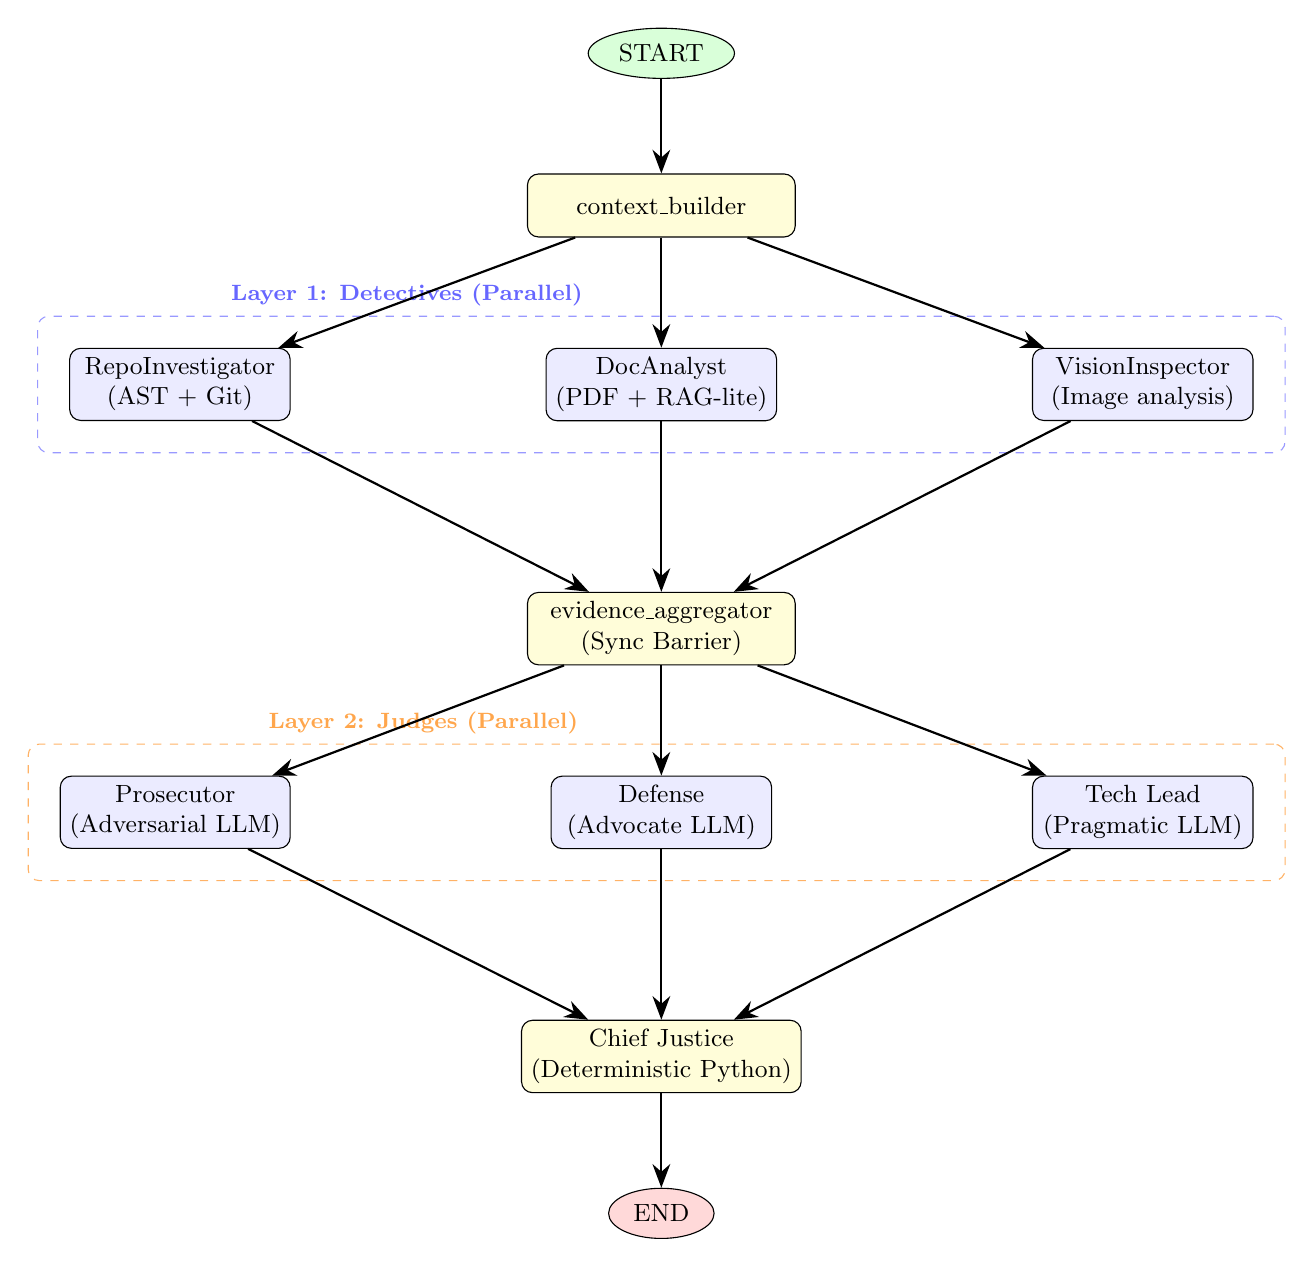
\begin{tikzpicture}[
  node distance=1.2cm and 2.0cm,
  every node/.style={font=\small},
  block/.style={rectangle, draw, rounded corners, minimum height=0.8cm, minimum width=2.8cm, align=center, fill=blue!8},
  sync/.style={rectangle, draw, rounded corners, minimum height=0.8cm, minimum width=3.4cm, align=center, fill=yellow!15},
  start/.style={ellipse, draw, minimum height=0.6cm, fill=green!15, align=center},
  endnode/.style={ellipse, draw, minimum height=0.6cm, fill=red!15, align=center},
  arr/.style={-{Stealth[length=3mm]}, thick}
]

% Nodes
\node[start] (start) {START};
\node[sync, below=of start] (ctx) {context\_builder};

% Detective layer
\node[block, below left=1.4cm and 3cm of ctx] (repo) {RepoInvestigator\\(AST + Git)};
\node[block, below=1.4cm of ctx] (doc) {DocAnalyst\\(PDF + RAG-lite)};
\node[block, below right=1.4cm and 3cm of ctx] (vis) {VisionInspector\\(Image analysis)};

\node[sync, below=4.5cm of ctx] (agg) {evidence\_aggregator\\(Sync Barrier)};

% Judge layer
\node[block, below left=1.4cm and 3cm of agg] (pros) {Prosecutor\\(Adversarial LLM)};
\node[block, below=1.4cm of agg] (def) {Defense\\(Advocate LLM)};
\node[block, below right=1.4cm and 3cm of agg] (tech) {Tech Lead\\(Pragmatic LLM)};

\node[sync, below=4.5cm of agg] (cj) {Chief Justice\\(Deterministic Python)};
\node[endnode, below=of cj] (end) {END};

% Edges
\draw[arr] (start) -- (ctx);
\draw[arr] (ctx) -- (repo);
\draw[arr] (ctx) -- (doc);
\draw[arr] (ctx) -- (vis);
\draw[arr] (repo) -- (agg);
\draw[arr] (doc) -- (agg);
\draw[arr] (vis) -- (agg);
\draw[arr] (agg) -- (pros);
\draw[arr] (agg) -- (def);
\draw[arr] (agg) -- (tech);
\draw[arr] (pros) -- (cj);
\draw[arr] (def) -- (cj);
\draw[arr] (tech) -- (cj);
\draw[arr] (cj) -- (end);

% Layer labels
\begin{scope}[on background layer]
  \node[draw=blue!40, dashed, rounded corners, inner sep=0.4cm, fit=(repo)(doc)(vis), label={[font=\footnotesize\bfseries, blue!60]above left:Layer 1: Detectives (Parallel)}] {};
  \node[draw=orange!60, dashed, rounded corners, inner sep=0.4cm, fit=(pros)(def)(tech), label={[font=\footnotesize\bfseries, orange!70]above left:Layer 2: Judges (Parallel)}] {};
\end{scope}

\end{tikzpicture}
\caption{Full StateGraph topology with two parallel fan-out/fan-in layers. Layer~1 uses deterministic Python tools; Layer~2 uses LLM-powered structured output. The Chief Justice applies deterministic conflict resolution.}
\label{fig:graph}
\end{figure}

\subsection{How Parallelism Works in LangGraph}

LangGraph achieves parallelism through its edge-based scheduling. When we write:

\begin{lstlisting}[caption={Fan-out wiring in \texttt{src/graph.py}}]
builder.add_edge("context_builder", "repo_investigator")
builder.add_edge("context_builder", "doc_analyst")
builder.add_edge("context_builder", "vision_inspector")
\end{lstlisting}

This tells LangGraph that all three nodes are ready to execute as soon as \texttt{context\_builder} completes. LangGraph runs them concurrently (using async or threading, depending on the runtime). The \texttt{evidence\_aggregator} node has three incoming edges:

\begin{lstlisting}[caption={Fan-in wiring in \texttt{src/graph.py}}]
builder.add_edge("repo_investigator", "evidence_aggregator")
builder.add_edge("doc_analyst", "evidence_aggregator")
builder.add_edge("vision_inspector", "evidence_aggregator")
\end{lstlisting}

LangGraph will not execute \texttt{evidence\_aggregator} until \emph{all three} upstream nodes have completed. The results from each Detective are merged into the shared state using the \texttt{operator.ior} reducer (for the \texttt{evidences} dict). This fan-in pattern is replicated for the Judicial Layer: three Judges fan out from \texttt{evidence\_aggregator}, and the \texttt{chief\_justice} node fans them in.

\subsection{Node Responsibilities}

\begin{longtable}{@{}p{3.5cm}p{2cm}p{7.5cm}@{}}
\toprule
\textbf{Node} & \textbf{Brain} & \textbf{Responsibility} \\
\midrule
\endhead
\texttt{context\_builder} & Python & Loads rubric dimensions from \texttt{rubric.json}, injects them into state. Entry point that feeds configuration to all downstream nodes. \\
\texttt{repo\_investigator} & Python (AST) & Clones the target repo into a sandboxed temp directory. Runs 7 forensic protocols: git history, state definitions, graph structure, tool safety, structured output, judicial nuance, chief justice synthesis. Produces \texttt{Evidence} objects per dimension. \\
\texttt{doc\_analyst} & Python (PyMuPDF) & Ingests the PDF report using a RAG-lite chunking approach (1000-char chunks). Searches for theoretical depth keywords, distinguishes substantive usage from buzzword dropping. Cross-references file paths mentioned in the report against the actual repo file list to detect hallucinated claims. \\
\texttt{vision\_inspector} & Python (stub) & Extracts images from the PDF and classifies diagram types. Currently a placeholder returning low-confidence evidence. Designed for future integration with a multimodal LLM. \\
\texttt{evidence\_aggregator} & Python & Synchronization barrier. Logs summary statistics (dimension count, evidence count, positive findings) but does not modify state. The actual merging happens through the \texttt{operator.ior} reducer. \\
\texttt{prosecutor} & LLM & Adversarial judge persona. Assumes the worst, scrutinizes for gaps. Default scoring range is 1--2 unless evidence is overwhelmingly positive. Uses \texttt{.with\_structured\_output(JudicialOpinion)} to enforce Pydantic validation on every LLM response. \\
\texttt{defense} & LLM & Advocate judge persona. Rewards effort, intent, and creative workarounds. Default scoring range is 4--5 if basic structure exists. Same structured output enforcement. \\
\texttt{tech\_lead} & LLM & Pragmatic judge persona. Focuses on ``does it work? is it maintainable?'' Starts at 3 and adjusts based on concrete technical findings. Same structured output enforcement. \\
\texttt{chief\_justice} & Python & Deterministic synthesis engine. Groups opinions by dimension, applies five conflict resolution rules (Section~\ref{sec:rules}), builds the final \texttt{AuditReport} with scores, dissent summaries, and a remediation plan. \\
\bottomrule
\end{longtable}


% ══════════════════════════════════════════════════════════
\section{The Judicial Layer: Dialectical Synthesis}

\subsection{Why Three Personas Instead of One Grader}

A single LLM evaluating code tends to produce bland, middle-of-the-road scores. Asking ``rate this code 1--5'' typically yields 3 or 4 regardless of quality. The dialectical approach forces the model into \emph{three distinct reasoning frames}:

\begin{itemize}
  \item The \textbf{Prosecutor} is instructed to assume the code is guilty until proven otherwise. Its system prompt says: ``Start from the assumption that the submission is lazy and has taken shortcuts. Your default score is 1--2. Only increase if the evidence is overwhelmingly positive.'' This persona is specifically tuned to look for missing features, security flaws, and structural problems.

  \item The \textbf{Defense} is instructed to be an advocate. Its prompt says: ``Look for creative workarounds, deep understanding, and effort. If the git history shows iteration and struggle, argue for higher scores. Your default is 4--5 if basic structure is present.'' This persona catches strengths that the Prosecutor would dismiss.

  \item The \textbf{Tech Lead} is the pragmatic middle ground. Its prompt says: ``Ignore the vibe. Does the code actually work? Is the architecture modular? Start at 3 and adjust based on concrete technical evidence.'' This persona serves as a tie-breaker.
\end{itemize}

We verified that the three prompt templates share \textbf{less than 50\% word overlap} (tested automatically in \texttt{test\_prompts.py}) to prevent ``Persona Collusion'' --- the failure mode where differently-named judges produce near-identical outputs because their prompts are too similar.

\subsection{Structured Output Enforcement}

Every Judge LLM call uses \texttt{ChatOllama.with\_structured\_output(JudicialOpinion)}. This means the LLM is constrained to return JSON matching the \texttt{JudicialOpinion} Pydantic schema:

\begin{lstlisting}[caption={JudicialOpinion schema enforced on every LLM call}]
class JudicialOpinion(BaseModel):
    judge: Literal["Prosecutor", "Defense", "TechLead"]
    criterion_id: str
    score: int = Field(ge=1, le=5)
    argument: str
    cited_evidence: List[str]
\end{lstlisting}

If the LLM returns malformed JSON (missing a field, wrong type, score outside 1--5), the system does not crash. Instead, it enters a \textbf{retry loop} (up to 2 retries) where a correction message is appended to the conversation: ``Your previous response did not match the required schema. Here is the exact schema you must follow: [schema].'' If all retries fail, the system falls back to a \textbf{neutral score of 3} with an argument explaining that the judge failed to produce a valid opinion. This graceful degradation ensures the pipeline always completes.


% ══════════════════════════════════════════════════════════
\section{The Chief Justice: Deterministic Conflict Resolution}
\label{sec:rules}

The Chief Justice is \textbf{not an LLM}. It is pure Python \texttt{if/elif/else} logic that implements five named rules from the rubric's \texttt{synthesis\_rules} specification.

\subsection{Rule 1: Security Override}

\textbf{Trigger:} The RepoInvestigator found evidence of \texttt{os.system()} or \texttt{shell=True} in the target codebase (a concrete AST finding), \emph{and} the dimension being scored is security-related.

\textbf{Effect:} The final score for that dimension is capped at 3, regardless of what the Defense argued. The rationale is that a confirmed security vulnerability cannot be offset by ``good effort.''

\textbf{Implementation:} The \texttt{\_has\_security\_violation()} function scans all Evidence objects for keywords like \texttt{os.system} and \texttt{shell=true} in evidence where \texttt{found=True}. This is a factual check on Detective output, not an interpretation.

\subsection{Rule 2: Fact Supremacy}

\textbf{Trigger:} The Defense scored a dimension $\geq 4$, but \emph{every} piece of Detective evidence for that dimension has \texttt{found=False}.

\textbf{Effect:} The Defense is overruled for ``hallucination.'' The weighted score is recalculated using only the Prosecutor (weight 0.40) and Tech Lead (weight 0.60), excluding the Defense entirely.

\textbf{Rationale:} If the Detectives found no supporting evidence (the file does not exist, the feature is not implemented), then the Defense cannot credibly argue for a high score. Facts override opinion.

\subsection{Rule 3: Functionality Weight}

\textbf{Trigger:} The dimension is \texttt{graph\_orchestration} (the architecture criterion).

\textbf{Effect:} The Tech Lead's weight increases from the default 0.40 to 0.60, while Prosecutor and Defense each drop to 0.20. For all other dimensions, the default weights are Prosecutor=0.30, Defense=0.30, TechLead=0.40.

\textbf{Rationale:} The rubric states that ``if the Tech Lead confirms the architecture is modular and workable, this carries the highest weight for the Architecture criterion.'' This rule implements that directive literally.

\subsection{Rule 4: Variance Re-evaluation}

\textbf{Trigger:} The spread between the highest and lowest judge scores exceeds 2 (e.g., Prosecutor=1, Defense=5).

\textbf{Effect:} The final score is pulled toward the median: $\text{final} = \lfloor(\text{weighted} + \text{median}) / 2\rfloor$. This dampens extreme disagreements without discarding any judge's input.

\textbf{Rationale:} High variance signals genuine ambiguity. Rather than letting either extreme dominate, we blend the weighted score with the statistical center.

\subsection{Rule 5: Dissent Requirement}

\textbf{Trigger:} Same as Rule~4 --- score variance exceeds 2.

\textbf{Effect:} The system generates a \texttt{dissent\_summary} string that documents each judge's score and a truncated version of their argument. This summary is included in the final report so the reader can understand \emph{why} the judges disagreed.

\textbf{Rationale:} The rubric requires that ``every criterion with a score variance $> 2$ must include an explicit dissent explanation.'' The dissent summary makes audit reports transparent and auditable.

\subsection{Score Calculation}

For each dimension, the base score is calculated as a weighted average:

$$
\text{weighted} = w_P \times s_P + w_D \times s_D + w_{TL} \times s_{TL}
$$

where $w_P, w_D, w_{TL}$ are the judge weights (default 0.30, 0.30, 0.40; architecture override 0.20, 0.20, 0.60) and $s_P, s_D, s_{TL}$ are the respective scores. The rules are then applied in sequence: security override caps, fact supremacy adjusts weights, variance re-evaluation blends with median. The final score is clamped to $[1, 5]$.


% ══════════════════════════════════════════════════════════
\section{Testing Strategy}

We used a test-driven development (TDD) approach throughout: tests were written alongside or before each module. As of the interim submission, the suite contains \textbf{165 tests} organized into 8 test files, all passing:

\begin{table}[h]
\centering
\caption{Test suite breakdown}
\begin{tabular}{@{}lrl@{}}
\toprule
\textbf{Test File} & \textbf{Count} & \textbf{Covers} \\
\midrule
\texttt{test\_state.py}           & 17 & Pydantic models, reducers, serialization \\
\texttt{test\_repo\_tools.py}     & 25 & AST parsing, git forensics, sandboxing \\
\texttt{test\_doc\_tools.py}      & 21 & PDF ingestion, keyword search, hallucination detection \\
\texttt{test\_detectives.py}      & 24 & Detective node functions, dimension filtering \\
\texttt{test\_graph.py}           & 20 & Graph topology, fan-out/fan-in, 9-node verification \\
\texttt{test\_prompts.py}         & 14 & Persona distinctness ($<$50\% overlap), format helpers \\
\texttt{test\_judges.py}          & 13 & Retry logic, mock LLM, structured output \\
\texttt{test\_chief\_justice.py}  & 31 & All 5 synthesis rules, report building \\
\midrule
\textbf{Total} & \textbf{165} & \\
\bottomrule
\end{tabular}
\end{table}

Key testing techniques include:
\begin{itemize}[nosep]
  \item \textbf{Self-referential testing:} \texttt{test\_repo\_tools.py} runs the AST analysis functions against the auditor's own source code, verifying they detect the actual Pydantic models and StateGraph wiring present in our codebase.
  \item \textbf{Mock LLM injection:} Judge tests use a \texttt{\_mock\_llm\_that\_returns()} factory that creates mock objects whose \texttt{.invoke()} method returns valid \texttt{JudicialOpinion} objects, allowing us to test the retry logic and node functions without making actual LLM calls.
  \item \textbf{Rule isolation:} Each of the 5 Chief Justice synthesis rules has dedicated tests that set up a specific conflict scenario (e.g., high variance, security violation) and verify that exactly one rule triggers with the expected effect.
\end{itemize}


% ══════════════════════════════════════════════════════════
\section{Current Implementation Status}

\begin{table}[h]
\centering
\caption{File-level implementation status}
\begin{tabular}{@{}llrl@{}}
\toprule
\textbf{Path} & \textbf{Status} & \textbf{Lines} & \textbf{Notes} \\
\midrule
\texttt{src/state.py}                  & Complete & 216  & All 5 Pydantic models + AgentState \\
\texttt{src/graph.py}                  & Complete & 121  & 9-node graph, 2 parallel layers \\
\texttt{src/prompts.py}                & Complete & 162  & 3 persona prompts, registry \\
\texttt{src/tools/repo\_tools.py}      & Complete & 1104 & 7 AST forensic protocols \\
\texttt{src/tools/doc\_tools.py}       & Complete & 440  & PDF ingestion, cross-reference \\
\texttt{src/tools/vision\_tools.py}    & Stub     & 88   & Returns low-confidence evidence \\
\texttt{src/nodes/detectives.py}       & Complete & 311  & 3 detective nodes \\
\texttt{src/nodes/judges.py}           & Complete & 200  & 3 LLM judge nodes + retry \\
\texttt{src/nodes/chief\_justice.py}   & Complete & 375  & 5 synthesis rules + report \\
\texttt{app.py}                        & Complete & 460  & Streamlit UI (3 tabs) \\
\texttt{rubric.json}                   & Complete & ---  & 10 dimensions, 5 rules \\
\texttt{pyproject.toml}               & Complete & ---  & uv-managed dependencies \\
\texttt{.env.example}                 & Complete & ---  & All env vars documented \\
\midrule
\textbf{Total source} & & \textbf{$\sim$3,500} & \\
\bottomrule
\end{tabular}
\end{table}


% ══════════════════════════════════════════════════════════
\section{Known Gaps and Plan for Final Submission}

Despite having all three layers implemented and passing 165 tests, several gaps remain:

\subsection{VisionInspector Is a Stub}

The \texttt{vision\_inspector} node currently extracts images from PDFs (via PyMuPDF) but classifies them with placeholder logic, returning \texttt{confidence=0.3} and a ``PENDING'' status. To make this production-ready, we plan to:
\begin{enumerate}[nosep]
  \item Integrate a multimodal LLM (such as \texttt{llama3.2-vision} or GPT-4o via API) to analyze extracted diagram images.
  \item Prompt the vision model with specific questions: ``Is this a LangGraph StateGraph diagram showing parallel fan-out/fan-in, or a generic box diagram?''
  \item Add classification logic to distinguish between accurate architecture diagrams, sequence diagrams, and misleading linear pipelines.
\end{enumerate}

\subsection{Git History Is Shallow}

The current commit history has only 3 commits (environment setup, Phase~0 structure, Phase~0+1 combined push). For the final submission, we plan to commit more incrementally to demonstrate the iterative development process that the rubric's ``Git Forensic Analysis'' dimension evaluates.

\subsection{Self-Audit Not Yet Generated}

The \texttt{audit/report\_onself\_generated/} directory exists but is empty. For the final submission, we will:
\begin{enumerate}[nosep]
  \item Run the full pipeline against our own repository.
  \item Commit the generated Markdown audit report.
  \item Analyze the results to identify and fix remaining weaknesses (the MinMax feedback loop).
\end{enumerate}

\subsection{Peer Audit Not Yet Conducted}

The \texttt{audit/report\_onpeer\_generated/} and \texttt{audit/report\_bypeer\_received/} directories are empty, pending peer assignment and the peer review cycle in the final phase.

\subsection{Conditional Error Edges}

The graph currently has no conditional edges for error handling (e.g., ``if clone fails, skip directly to the aggregator with empty evidence''). This is a robustness gap: if the target repo URL is invalid or the PDF is corrupted, individual detective nodes handle errors internally via try/except, but there is no graph-level short-circuit. We plan to add conditional edges for the final submission.

\subsection{LangSmith Tracing Integration}

The \texttt{.env.example} includes \texttt{LANGCHAIN\_TRACING\_V2=true} and \texttt{LANGCHAIN\_API\_KEY}, and the infrastructure is in place via \texttt{python-dotenv}. However, we have not yet run a traced end-to-end execution. For the final submission, we will provide a LangSmith trace link showing the full reasoning loop.

\subsection{Dockerization}

No \texttt{Dockerfile} exists yet. For the final submission, we plan to containerize the application for reproducible execution.


% ══════════════════════════════════════════════════════════
\section{Technology Stack}

\begin{table}[h]
\centering
\caption{Core dependencies and their roles}
\begin{tabular}{@{}llp{7cm}@{}}
\toprule
\textbf{Package} & \textbf{Version} & \textbf{Role} \\
\midrule
\texttt{langgraph}        & 1.0.9  & StateGraph definition, parallel node execution, edge-based orchestration \\
\texttt{langchain-core}   & 1.2.15 & Message types (SystemMessage, HumanMessage), base abstractions \\
\texttt{langchain-ollama} & 1.0.1  & \texttt{ChatOllama} with \texttt{.with\_structured\_output()} for local LLM inference \\
\texttt{pydantic}         & 2.12.5 & Typed data models, field validation, JSON schema generation \\
\texttt{pymupdf}          & 1.27.1 & PDF text extraction, image extraction (PyMuPDF/fitz) \\
\texttt{streamlit}        & 1.54.0 & Web UI for interactive auditing \\
\texttt{python-dotenv}    & 1.2.1  & Secure environment variable management \\
\texttt{pytest}           & 9.0.2  & Test framework \\
\texttt{uv}               & 0.10.0 & Dependency management and lockfile \\
\bottomrule
\end{tabular}
\end{table}

We use \textbf{Ollama} for local LLM inference rather than cloud APIs. This means the Judicial Layer runs entirely on-premise, requiring no API keys for the LLM itself. The available models are \texttt{qwen3-coder:480b-cloud} and \texttt{deepseek-v3.1:671b-cloud}, configurable via the \texttt{OLLAMA\_MODEL} environment variable.

% ══════════════════════════════════════════════════════════
\section{Repository Structure}

The submitted repository contains the following deliverable files:

\begin{lstlisting}[language={}, caption={Repository file tree}]
swarm-auditor/
|-- app.py                         # Streamlit frontend
|-- rubric.json                    # Machine-readable rubric (v3.0.0)
|-- pyproject.toml                 # uv-managed dependencies
|-- uv.lock                        # Locked dependency versions
|-- .env.example                   # Environment variable template
|-- README.md                      # Setup + run instructions
|-- src/
|   |-- __init__.py
|   |-- state.py                   # Pydantic models + AgentState
|   |-- graph.py                   # 9-node StateGraph
|   |-- prompts.py                 # 3 judge persona prompts
|   |-- tools/
|   |   |-- __init__.py
|   |   |-- repo_tools.py         # Sandboxed git + AST analysis
|   |   |-- doc_tools.py          # PDF ingestion + cross-ref
|   |   |-- vision_tools.py       # Image analysis (stub)
|   |-- nodes/
|       |-- __init__.py
|       |-- detectives.py         # 3 detective LangGraph nodes
|       |-- judges.py             # 3 judge LangGraph nodes
|       |-- chief_justice.py      # Deterministic synthesis
|-- tests/
|   |-- __init__.py
|   |-- test_state.py             # 17 tests
|   |-- test_repo_tools.py        # 25 tests
|   |-- test_doc_tools.py         # 21 tests
|   |-- test_detectives.py        # 24 tests
|   |-- test_graph.py             # 20 tests
|   |-- test_prompts.py           # 14 tests
|   |-- test_judges.py            # 13 tests
|   |-- test_chief_justice.py     # 31 tests
|-- audit/                         # Empty; populated at final
|-- reports/
    |-- interim_report.pdf         # This document
\end{lstlisting}


% ══════════════════════════════════════════════════════════
\section{Conclusion}

The Swarm Auditor implements the full ``Digital Courtroom'' architecture specified in the FDE/TRP1 Week~2 challenge. The Detective Layer provides objective, AST-based forensic evidence. The Judicial Layer generates structured, adversarial opinions through three distinct LLM personas. The Chief Justice resolves conflicts using deterministic Python rules that faithfully implement the rubric's synthesis specifications.

The system is backed by 165 passing tests, type-safe Pydantic models throughout, sandboxed execution for security, and a clean separation between facts (Detectives), opinions (Judges), and decisions (Chief Justice). The remaining gaps --- VisionInspector integration, self-audit generation, peer review execution, conditional error edges, and Dockerization --- are well-defined and planned for the final submission.


\end{document}
